\documentclass[paper=a4, fontsize=11pt]{scrartcl} % A4 paper and 11pt font size
\usepackage{hyperref}
\usepackage{movie15}
\usepackage{graphicx}
\hypersetup{hidelinks}
\usepackage{graphics}
\usepackage{geometry}
\usepackage{url}
\geometry{verbose,letterpaper}
\usepackage[T1]{fontenc} % Use 8-bit encoding that has 256 glyphs
\usepackage{fourier} % Use the Adobe Utopia font for the document - comment this line to return to the LaTeX default
\usepackage[english]{babel} % English language/hyphenation
\usepackage{amsmath,amsfonts,amsthm} % Math packages

\usepackage{lipsum} % Used for inserting dummy 'Lorem ipsum' text into the template
%\usepackage{movie15}
\usepackage{sectsty} % Allows customizing section commands
\allsectionsfont{\centering \normalfont\scshape} % Make all sections centered, the default font and small caps

\usepackage{fancyhdr} % Custom headers and footers
\pagestyle{fancyplain} % Makes all pages in the document conform to the custom headers and footers
\fancyhead{} % No page header - if you want one, create it in the same way as the footers below
\fancyfoot[L]{} % Empty left footer
\fancyfoot[C]{} % Empty center footer
\fancyfoot[R]{\thepage} % Page numbering for right footer
\renewcommand{\headrulewidth}{0pt} % Remove header underlines
\renewcommand{\footrulewidth}{0pt} % Remove footer underlines
\setlength{\headheight}{13.6pt} % Customize the height of the header

\numberwithin{equation}{section} % Number equations within sections (i.e. 1.1, 1.2, 2.1, 2.2 instead of 1, 2, 3, 4)
\numberwithin{figure}{section} % Number figures within sections (i.e. 1.1, 1.2, 2.1, 2.2 instead of 1, 2, 3, 4)
\numberwithin{table}{section} % Number tables within sections (i.e. 1.1, 1.2, 2.1, 2.2 instead of 1, 2, 3, 4)

\setlength\parindent{2em} % Removes all indentation from paragraphs - comment this line for an assignment with lots of text

%----------------------------------------------------------------------------------------
%	TITLE SECTION
%----------------------------------------------------------------------------------------

\newcommand{\horrule}[1]{\rule{\linewidth}{#1}} % Create horizontal rule command with 1 argument of height

\title{	
\normalfont \normalsize 
\textsc{Southern University of Science and Technology, Dept of Biomedical Engineering} \\ [25pt] % Your university, school and/or department name(s)
\horrule{0.5pt} \\[0.4cm] % Thin top horizontal rule
\huge Presentation of functional ultrasound imaging\\ % The assignment title
\horrule{2pt} \\[0.5cm] % Thick bottom horizontal rule
}

\author{Dong Haowen \& Ye Yuming} % Your name

\date{\normalsize\today} % Today's date or a custom date

\begin{document}

\maketitle
We don't want the length of this manuscript to be too long, so many of the pictures and videos mentioned are not put in, but they are easy to correspond in the PPT version.

All of our PPT and manuscript were generated from Latex. For more details and pictures. Please visit our website:
 \url{https://github.com/fonding/Principle-of-medical-imaging}

*contact us at: idarrendong@gmail.com

\section{History of ultrasound imaging}

Built in 1950s and extensively developed and applied in 1970s, ultrasound imaging is now widely used in many fields. 

In 1942, K. T Dussik developed A mode ultrasound and detect the brain. In 1954, Donald used ultrasound imaging in gynecologic examination and in 1965, Lallagen use D mode ultrasound imaging to test fetal heart rate and vascular disease. Nearly 30 years, the medical ultrasonic diagnosis technology happened again and again to a revolutionary leap. Interventional ultrasound gradually popularized in the 1980s, the body cavity and the application of intraoperative probe enlarged the scope and the quality of diagnosis. In 1990s, intravascular ultrasound, three-dimensional imaging and the application of new type of acoustic contrast agent made the ultrasonic diagnosis raise on a new step. 

The general trend of development is from static to dynamic images (rapid imaging), from black and white to colorful images, from two-dimensional to three-dimensional images, from reflection method to transmission method. In order to get a specific ultrasonic signal, to achieve the purpose of quantitative, specific diagnosis, scientists had made huge efforts. 

However, ultrasound imaging also faced with many problems like lack of resolution. Thus, functional ultrasound imaging and ultrafast ultrasound localization microscopy rise in response to the proper time and conditions. 



%------------------------------------------------
\section{Principles}
For explaining functional ultra-sound imaging.
We selected two related paper to explain it. One is called: Functional ultrasound imaging in brain. The other is: Ultrafast Ultrasound localization microscopy for deep super-resolution vascular imaging.

Both of them put forward a novel method to achieve functional ultrasound imaging. In order to explain these two different methods clearer, we separate the principle section into two parts. Each correspond two a specific method.
\subsection{Function ultrasound imaging in brain}

Before we enter into the functional ultrasound imaging in brain, we first review what contribute to the ultrasound imaging’s resolution. The first are the wave length. The resolution is better when the ultrasound’s wavelength gets shorter. The second factor are focusing size, when the focus effect is good enough, the resolution gets better. And also, Signal attenuation is a non-ignorable thing when apply imaging system. 

Actually, if one imaging method was determined, there is a balance between its spatial and time resolution. Traditional ultrasound imaging way is by line scanning. The first functional ultrasound imaging approach is try to innovative scanning mode: If the scan method is replaced by plane scan, the time resolution of imaging will be greatly improved, then find a way to sacrifice temporal resolution for spatial resolution.

The basic principle of plane scanning was described here. These two formulas were used to demonstrate the time that the sound needed to travel the tissue and back to the acceptor. Compare formula (1) with (2)(PPT version), the surplus item in formula (2) is related to $\alpha$, which is the plane’s slope reference to the tissue. 

As for whole image, we treat is as a function of x, z and $\alpha$. The result is related to detector’s position and subject’s position also the plane slope. If the slope was changed from one degree, a set of new image’s data was produced. If the slope was changed for N times. And Simply add them up, the final result will only relate to x and z, which is the position of subject.

There is a better way to process these data. Base on the “Probability and Statistics”, a series of image’s matrix correspond data can be created as a $\chi^{2}$ distribution. The number of images(slopes) is its degree of freedom. According to one of $\chi^{2}$ distribution’s characteristic, as degree of freedom gets higher, it’s distribution will be closer to Gaussian distribution. The center mean value was treated as compound image’s gray value of its original location. By applying this method, ‘’part of time resolution is converted to spatial resolution’’.

Theoretically, the velocity of ultrasound in brain is about 1540m/s. Assume the imaging depth is 5cm and we take 15 angles of deflection from -7 to 7 to create an image. The frequency of one single picture is 1540m/s / 0.1m = 15400Hz, we divide it by 15, the theoretical imaging frequency is found about 1026Hz. However, for traditional 128-line focused ultrasound frame, it’s imaging frequency is about 120Hz.

After combining plane scanning and multi-frame synthesis technology, this ultrasound imaging system can achieve relative high resolution with very high time resolution, it can be applied to monitor brain’s activity in some situation. Here is a video for example to monitor mouse brain’s activity.

However, as shown in video, the brain is shown in heat map form. How can it transform into that form. Basically, it’s accomplished by Pearson’s correlation coefficient. Calculate one frame’s correlation coefficient with previous one. Following is an example, if two matrices possess this coefficient higher than a threshold value, this means there is no obvious difference between this two moments. But if their correlation coefficient lowers that this value, it means that there is a significance different, red color was cover on this area and transfer black/white picture into activation map.

In conclusion for this part, here is another video for comparing this imaging method with traditional method.

\subsection{Ultrafast ultrasound localization microscopy}
For another ultrasound imaging approach – ultrafast ultrasound localization microscopy. There is a short story for its discovery. Nobel prize was award to three scientists who contributions to optical super-resolution microscopy- PALM. 

The basic principle of PALM is to active small number of fluorescent dots at a time. Then record its position base on airy disk’s center. Bleach them and repeat these procedures. During this process, one single airy disk was abstract to a single point, which is correspond to its center. In principle, this creative idea can bring resolution to angstrom scale.

Inspired by this imaging technology, Tanter used the similar method developed super-resolution ultrasound imaging system. Here is a picture of blood flow in the brain of rats by using this technology. The red color indicates that blood flows from top to bottom and blue color means blood flow from bottom to top.

There is a substance needed in PLAM – “fluorescence polymer dots”. Correspondingly, a special contrast agent was used in ultrasound imaging method – ‘micro-vesicle’. Microvesicle can be injected into rat’s blood and flow with blood. However, it’s not stable enough, some vesicles will burst and causing a wavelength level change in image if ultrasound focused on this area. In similar way, these changes will be recorded and abstracted to an ideal point, increasing image resolution.

Due to the limitation of other factors like detectors’ sensitivity. There are no enough data for processing Gaussian fit. Interpolation method was used in image processing stage. Bilinear interpolation shows the most basic idea of interpolation. There are 4 points already known. The value of P point can be determined by following procedures: Assume there is a linear function between Q12 and Q22, calculate out R2 value and then calculate R1 by using the same method. Suppose linear relationship also suitable for R1 and R2, then P value could be find out. Theoretically, it could be applied to find every point in this plane. 

Thus, the unknown points are completed, and the image data becomes more. It much suitable to use Gaussian fit find its center.
Finally, this picture shows how the blood flow velocity is figured out by this method: Calculate the distance between each Gaussian center for two pictures next to each other in time, dividing it by time interval, the blood velocity is found out. 

This super resolution ultrasound imaging method provides high resolution while also provides information about blood flow in the tiny blood vessels in brain. It has the potential to play a role in early cancer screening and other mental disease research.
Then, it goes to application and prospect part.


%----------------------------------------------------------------------------------------
%	PROBLEM 2
%----------------------------------------------------------------------------------------
\section{Comparison and achievement of functional ultrasound imaging}
To begin with, the comparison of traditional Doppler ultrasound imaging and functional ultrasound imaging. One of the major limitations of conventional doppler ultrasound imaging for these images is undersensitivity, which makes blood flow in small vessels cannot be detected. However, the major hemodynamic reactions occur in small blood vessels. 

The following figure shows some difference of parameters of focused method (traditional ultrasound imaging) and compound method (functional ultrasound imaging). The main difference is the number of frames under the same sampling frequency and the same sampling time, in which obtained by functional ultrasound is 8 times higher than that of traditional doppler ultrasound.
\begin{figure}[htbp]
	\centering
	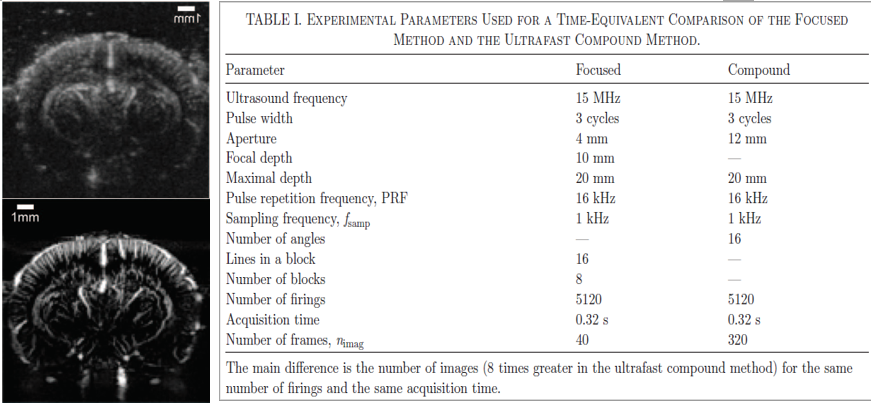
\includegraphics[width=1\linewidth]{im4}
	%	\caption{}
	%	\label{fig:im4}
\end{figure}

What’s more, the graphs on the left side show the quality difference of them. Functional ultrasound imaging has better signal-to-noise ratio and higher resolution. Functional ultrasound imaging uses 15-MHz ultrasonic probe which allows it to detect a whole mice brain map in a resolution of 100*100 square micron, 200 microns in thickness and a penetration depth greater than 2cm and it only takes 200 milliseconds. 
\section{Applications of functional ultrasound imaging}

\begin{itemize}
	\item Small animal imaging. Small animals have thinner skulls, so functional ultrasound imaging with an ultralight probe can apply non-invasive animal experiments without contrast agents, during which the brain activity of small animals in the process of behavior can be monitored in real time. 
	\item Neonatal pediatric neurology. The brain of premature infants may have developmental problems. Some premature infants may suffer from epilepsy due to blood vessel blockage. Functional ultrasound imaging during the seizure can better understand the neonatal seizure. Because functional ultrasound imaging is a clinical imaging method, it is possible to replace functional MRI in many clinical situations, which is difficult to be replaced nowadays.
	\item Intraoperative functional ultrasound imaging in adults. Now most brain tumors are detected using ultrasound or ultra-fast doppler imaging. Functional ultrasound imaging helps doctors map specific functional areas of the cortex during surgery. For example, the Electrical stimulation of the cerebral cortex (ESM) is the golden standard to locate the brain regions. However, it is far from perfect. It will cause pain, epilepsy and some nervous system diseases. Functional ultrasound imaging was used to determine brain activity areas according to the increase in cerebral blood volume caused by neurovascular coupling. This allows the functional areas of the brain to be identified in real time, noninvasively, and in high resolution.
\end{itemize}
(More about Neuro vascular coupling regulation mechanism: There are sophisticated neurovascular regulatory mechanisms in brain tissue that stabilize the energy and oxygen required for the normal functioning of the brain. In physiological state, this neural-vascular coupling regulation mechanism, also known as functional hyperemia, is the basis of brain functional imaging signals.)

\section{Comparison and achievement of ultrafast ultrasound localization microscopy}
Ultrafast ultrasound localization microscopy broke the limitation of resolution and it achieves one tenth of the wavelength. Optical microscopes can also achieve such high resolution, they developed rapidly recently, like super-resolution imaging (PALM and STORM) dramatically increased the resolution by an order of magnitude. 

The incomparable advantage of ultrasound is that it can penetrate organs without losing coherence, and is much less affected by the process of being de-correlated in the body. In traditional clinical ultrasound imaging applications, resolution is related to ultrasound frequency and inversely proportional to penetration depth. However, the resolution of ultrasound is affected by the diffraction limit, so the resolution and penetration need to be balanced. 

However, in ultrafast ultrasound location imaging, the resolution is related to the signal-to-noise ratio, the bandwidth of backscatter echoes and the number of array elements used in beam forming. It shows that very high resolution can be achieved in clinical applications, even down to the organs. Reported by the researcher, an image of a blood vessel with a resolution of 10 microns in the brain of a rat only takes 10 seconds to build up with, which is the highest resolution ever achieved by any technology. 

In fact, the thickness of human capillary is 6 to 9 microns. The contrast agent microbubbles used in Ultrafast ultrasound localization microscopy is around 2 microns. It gives ultrafast ultrasound localization microscopy broad possibilities because it can theoretically see any tiny capillaries within a certain depth range. 

In the future, ultrafast ultrasound localization microscope may become the most basic tool to understand and diagnose various disease processes that change microvascular blood flow. 

\section{Applications of ultrafast ultrasound localization microscopy}
\begin{itemize}
\item Monitor tumor status. When tumor growing, capillaries will grow towards the tumor and surround it, forming peripheral vascular network and offering nutrition. Early tumors can affect the direction of normal peripheral blood vessels. Thus, Ultrafast ultrasound localization microscopy can help doctor find the location of tumor and the specific shape of it. One example is that tracking the growth of new blood vessels around the tumor helps predict the growth rate of the tumor.  
\item Detecting coronary microvascular disease. On one hand, coronary microvasculature accounts for more than 95\% of the total coronary artery tree, but it cannot be shown by conventional contrast. There are data show that symptoms of chest pain patients with normal coronary angiography have 50\% to have coronary microvascular diseases. On the other hand, the treatment effect cannot be directly quantified, and doctors also measure the extent of the disease indirectly by measuring the ability of coronary blood flow to increase. Applying ultrafast ultrasound localization microscopy, more sophisticated and quantizable treatment can be applied to patients. It can bring great help to the detection and treatment of coronary microvascular disease. 
\end{itemize}

\section{Epilogue}
That's all about our presentation details. Thanks for your listening! References are available in PPT version. 


\end{document}